\documentclass[10pt,conference,compsocconf]{IEEEtran}

%Deadline: April 8, 2015
%Call for papers: http://www.computer.org/web/computingnow/swcfp6

\usepackage{url}
\usepackage[table,xcdraw]{xcolor}
\usepackage{eurosym}
\usepackage{amsfonts}
\usepackage{balance}
\usepackage{cite} %this package is awesome - it reorders lists of citations to be in numeric order
\usepackage{pifont}
\usepackage{eqparbox}

% Tables
\usepackage{booktabs}
\usepackage{pbox}
\renewcommand{\arraystretch}{1.2} 

%Images
\usepackage[pdftex]{graphicx}
\graphicspath{ {}{img/} }
\DeclareGraphicsExtensions{.pdf,.jpg,.png}

\hyphenation{second-ly ap-pen-dix}

\clubpenalty = 10000
\widowpenalty = 10000
\displaywidowpenalty = 10000

\newcommand{\todo}[1]{\textbf{TODO: #1}}

\begin{document}
%
% paper title
% can use linebreaks \\ within to get better formatting as desired
\title{Smell Detection and Refactoring in End-User Programming Languages}
%\title{Perspectives on End-User Refactoring: Past, Present, and Future}

\author{\IEEEauthorblockN{Felienne Hermans, David Hoepelman}
\IEEEauthorblockA{Delft University of Technology\\
Mekelweg 4\\
2628 CD Delft, the Netherlands\\
f.f.j.hermans@tudelft.nl}


\and
\IEEEauthorblockN{Kathryn T. Stolee}
\IEEEauthorblockA{Iowa State University\\
209 Atanasoff Hall\\
Ames, IA 50011-1041\\
kstolee@iastate.edu}
}

\maketitle


\begin{abstract}
In the workforce today, millions of people program without degrees or professional training in software development. 
These end-user programmers write code that designs hardware circuits, collects web information, and impacts business decisions. 
Software engineering research, an in particular refactoring, has traditionally focused on professional, and often object-oriented, programming languages, 
Yet, other domains and languages also suffer from code smells in need of refactoring. 
In this work, we explore recent research in three end-user domains and languages, spreadsheets in Microsoft Excel, web mashups in Yahoo!\ Pipes, and system designs in National Instruments' LabVIEW. 
%Smell detection and refactoring research in these three languages share many commonalities, stemming from the fact that they are all dataflow languages.  
Through exploring the commonalities and differences among the domains, we 1)~show how these end-user domains benefit from prior research in refactoring for object-oriented languages, 2)~discuss unique smell detection and refactoring opportunities for these domains and how they can translate to professional languages, and 3)~identify future opportunities for smell and refactoring research in these studied domains as well as other domains of end-user programming languages. 
\end{abstract}


\begin{IEEEkeywords}
code smells;
end-user programming;
refactoring;
\end{IEEEkeywords}

\section{Introduction}
The number of end-user programmers is said to greatly exceed the number of professional programmers. ``The proportion of American end user workers reporting they \emph{do programming} has remained relatively constant, rising from around 10\% in 1989 to only around 15\% in 2001''~\cite{Scaf2005} This 15\% of 2001 totals to about 11 million end users, while the number of professional developers was estimated at 3 million for the same period~\cite{Scaf2005}.
%These statistics seem a little dated... is there anything more recent?

End-user programmers perform a wide variety of tasks within their organizations, ranging from building or maintaining applications to simple data manipulation in a spreadsheet. While performing these tasks, end-user programmers face many of the challenges of professional developers, such as identifying faults, debugging, or understanding code written by someone else~\cite{Ko2011}.

Similar to code written by professional developers, end-user artifacts may have a long life-span. In fact, a 2011 case study showed that spreadsheets have an average lifespan of 5 years~\cite{Hermans2011}. During this long lifespan, end-user artifacts are modified, often by different people. This makes them, like source code artifacts, vulnerable to \emph{smells}. 

Smells in end-user programming have been a topic of research over the past few years. Most notable are structural smells in Yahoo!\ Pipes web mashups~\cite{Stolee2011} and  Excel spreadsheets \cite{Hermans2012inter} and performance smells in LabVIEW code \cite{chambers2013smell}.
Experiments in all these areas have shown that end-user programmers understand smells and often prefer versions of their code that are non-smelly.
Alleviating those smells can be achieved with refactoring.
%, which leads to the topic of this paper: \emph{what general concepts can we recognize over all types of end-user smell detection and refactoring approaches?}

%love this addition! I just moved it a bit for better flow. 
The applicability of smells, originally created to detect weaknesses in source code, to other domains shows how powerful the concept is. Furthermore, studying the smells in a fresh context  provides new insight on how to use smells in software engineering and  even suggests new types of smells. This is what we study in this paper.
The contributions of this work are:

\begin{itemize}
%	\item Synthesis of recent research in smell detection and refacotring for end-user programming languages
%	\item Motivation for the study of smells and refactoring for end-user programming languages based on empirical evidence
	\item Synthesis and catalog of object-oriented-inspired code smells  and refactoring in end-user programs
	\item Discussion of how smells and refactoring in  end-user domains may translate to professional languages
	\item Identification of future opportunities for smell detection and refactoring in end-user programming domains
\end{itemize}


\section{Background}
\label{sec:background}


Refactoring was first introduced as a systematic way to restructure source code and facilitate software evolution and maintenance~\cite{Opdyke:1992:ROF:169783, Griswold:1993:AAP:152388.152389}. In 1999, Martin Fowler introduced the concept of code smells for object-oriented (OO) languages~\cite{Fowl1999}. 
%Refactoring, improving the internal composition of a software program without altering its functionality or output \todo{quote a definition}, has been a part of software engineering since at least 1989 \cite{arnold1989software}, but was popularized by Fowler's 1999 "Refactoring: Improving the design of existing programs" \cite{fowler1999refactoring}. 
According to Fowler, code smells indicate suspicious or weak parts that the developer might want to change in order to improve readability and minimize the chance of future errors.
``A code smell is a surface indication that usually corresponds to a deeper problem in the system,'' says Fowler. For professional programmers, refactoring code is usually motivated by noticing a code smell, which signals the opportunity for improvement.

The taxonomy of smells outlined in Fowler's text pertained exclusively to object-oriented code, and professional programming languages were focus  for at least the first decade of refactoring and code smell research~\cite{Mens:2004:SSR:972215.972286}.
Since 2011, however, refactoring and smell definitions have been adapted and extended to other 
programming language paradigms, including web mashups~\cite{Stolee2011, StoleeTSE2013}, Excel spreadsheets~\cite{Hermans2011, Hermans2012inter, hermans2014bumblebee}, and LabVIEW programs~\cite{chambers2013smell}, all of which are end-user programming domains. 
%Further, these smells can be addressed using refactorings that, like the refactorings for professional programming languages, remove the smell while maintaining the code's behavior. 
%Like source code produced by professional developers, programs made by end-users can also contain smells.

%This is the same in end-user development, and as such we will first discuss the research on end-user development smells.
More importantly, researchers have  found that code smells matter to end-user programmers.
When presented with Yahoo!\ Pipes web mashups with and without smells, a significant majority of end-user programmers preferred the pipes without smells~\cite{StoleeTSE2013}.
In a field study done with 10 spreadsheet users at an investment bank, users agreed smells could reveal actual errors in their spreadsheets\todo{~\cite{}}.
When presenting LabVIEW users with information about code smells in their programs, all 13 participants were able to identify the problems and 12 were able to fix the problem~\cite{chambers2013smell}.
Considering the large number of end-user programmers, the longevity of their artifacts, and the real impact of smells on understandability, errors, and performance, supporting end-user programmers in code smell detection and refactoring is valuable. 

In this work, we explore past research in three end-user programming domains and languages: spreadsheets in Microsoft Excel, web mashups in Yahoo!\ Pipes, and visual system design in National Instruments' LabVIEW. Furthermore we identify future opportunities for smell and refactoring research in these and other end-user programing domains. Here, we briefly explore each language  before presenting the relevant code smells in  Section~\ref{sec:smells} and refactorings in Section~\ref{sec:refactoring}.

\paragraph{Excel}

\begin{figure}
\caption{Microsoft Excel 2013 showing a spreadsheet}
\centering
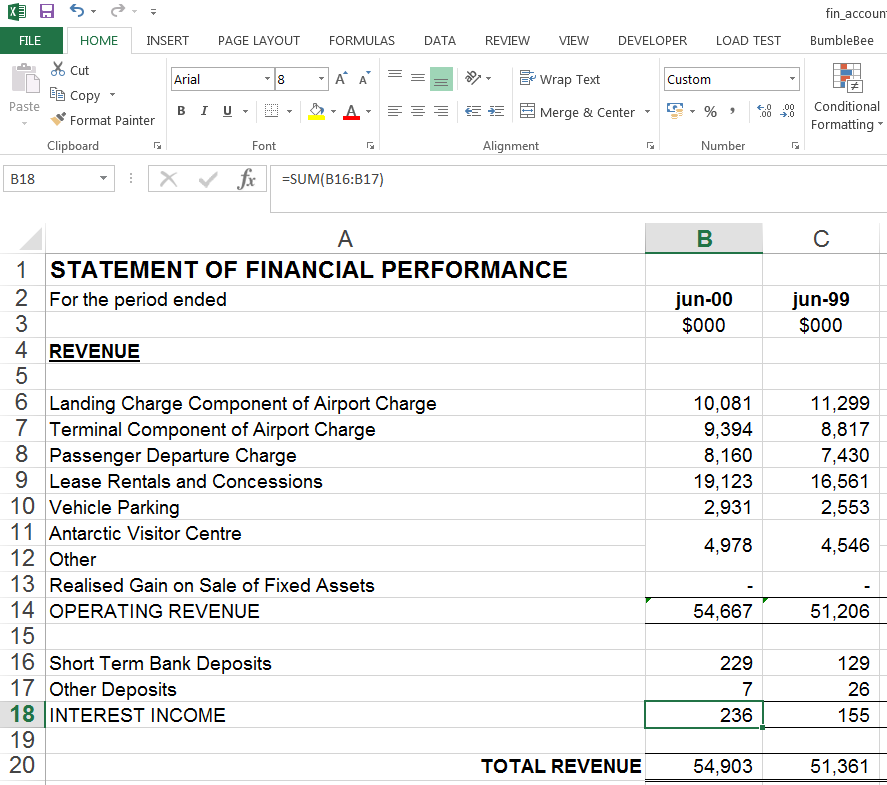
\includegraphics[width=\columnwidth]{excel-2}
\label{fig:spreadsheetexample}
\end{figure}

Spreadsheets are very commonly used in businesses, from inventory administration to educational applications and from scientific modeling to financial systems. Winston ~\cite{Wins2001} estimates that 90\% of all analysts in industry perform calculations in spreadsheets. Especially in the financial domain, spreadsheets are the way to perform modeling and programming. Panko~\cite{Pank2006} estimates that 95\% of U.S. firms, and 80\% in Europe, use spreadsheets in some form for financial reporting. 

In modern spreadsheet programs, a \textit{cell} can contain a single \textit{formula} which performs a calculation, and a table of cells is bundled in a \textit{worksheet}.
A \textit{workbook} consist of a collection of worksheets.
Formulas can reference other cells in the same or in a different worksheet.
References to a different workbook are possible but less common.


\paragraph{Yahoo!\ Pipes}
A web mashup is a program that collects and combines information from various
sources. 
In  Yahoo!\ Pipes, the information comes from RSS feeds. Figure~\ref{fig:ypexample} shows an example Yahoo!\ Pipes program with five RSS feed data sources, each in a \emph{Fetch Feed} module, feeding to a \emph{Union} module that concatenates the feeds, a \emph{Truncate} module that limits the number of items to 15 prior to the final \emph{Pipe Output}. 
Abstraction is possible in Yahoo!\ Pipes through the use of a \emph{subpipe} module, which allows a programmer to insert a different pipe as a subroutine, appearing like a standard module with a link to the source. 

\begin{figure}
\caption{Example of a program in Yahoo!\ Pipes}
\centering
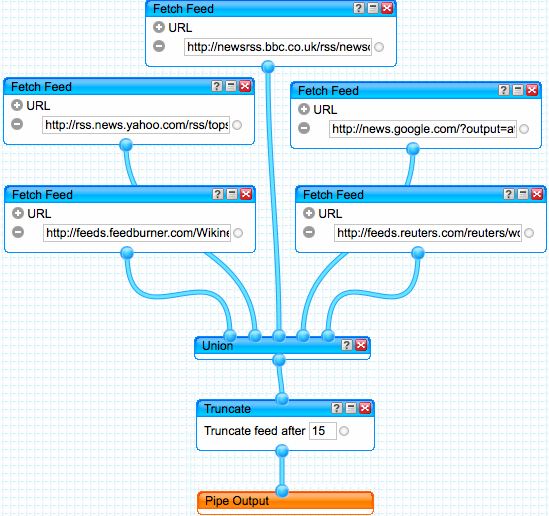
\includegraphics[width=\columnwidth]{yp-1}
\label{fig:ypexample}
\end{figure}


\paragraph{LabVIEW}
\begin{figure}
\caption{Example of a G program from the LabVIEW manual}
\centering
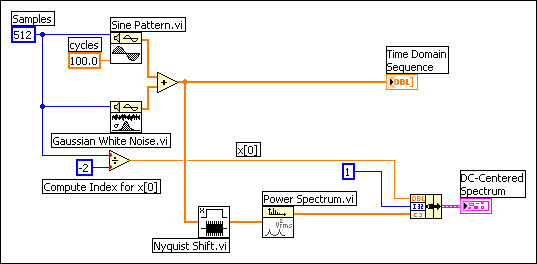
\includegraphics[width=\columnwidth]{labview-1}
\label{fig:labviewexample}
\end{figure}

LabVIEW is a proprietary, visual hardware system design environment that features the visual programming language ``G'' as one of its primary features.
An example of a G program can be found in Figure \ref{fig:labviewexample}.
G is a dataflow language which means a program is represented as a directed graph where data ``flows'' between nodes through their edges.
As such the two most important primitives in G are the edges called \textit{wires} and nodes called \textit{virtual instruments}.
VI's are very similar to functions, because they perform an operation on inputs and provide outputs.
Wires with no source VI are inputs and wires without a destination VI are outputs. 


\section{Smells in end-user programs}
\label{sec:smells}
\todo{We need to decide if we refer to smell names With Camel Case or lower case and be consistent.}
Research into end-user programming smells has had two approaches, which are not mutually exclusive.
The first approach is to take existing smells for OO programming languages, usually those defined by Fowler~\cite{Fowl1999}, and transform them to be applicable to the end-user environment \cite{Hermans2012inter,Hermans2012intra,Stolee2011,StoleeTSE2013, chambers2013smell}.
The second approach is to define smells tailored to the end-user environment.
This can be done by interviewing experienced end-users to see which smells they perceive \cite{chambers2013smell}, by looking at user reports like forum or newsgroup posts~ \cite{badame2012refactoring,chambers2013smell}, or by analyzing publicly available artifacts \cite{Stolee2011,StoleeTSE2013}.

This section provides an overview of different smells that researchers have found to be applicable to end-user artifacts using both the above described approaches and proposes future directions for smell detection in these domains. 


%\begin{table}
%\caption{OO Code Smells in End-User Programs
%\label{table:oosmells}}
%\begin{tabular} {| l | l | l | l |}
%\hline
%\textbf{Smell} & \textbf{Excel} & \textbf{Yahoo!\ Pipes} & \textbf{LabVIEW} \\ \hline
%
%Feature Envy & ~~ \ding{51}\cite{Hermans2012inter} & ~~ \ding{51}*& ~~  \\ 
%Long Method & ~~ \ding{51}\cite{Hermans2012intra} & ~~ \ding{51}* & ~~ \ding{51}*\\
%Message Chain & ~~ \ding{51} \cite{Hermans2012intra} & ~~ & ~~ \ding{51} \cite{chambers2013smell} \\
%Inappropriate Intimacy & ~~ \ding{51} \cite{Hermans2012inter} & ~~ \ding{51}*& ~~  \\ 
%Middle Man & ~~ \ding{51} \cite{Hermans2012inter} & ~~ \ding{51} \cite{StoleeTSE2013}  & ~~  \\
%Shotgun Surgery & ~~ \ding{51} \cite{Hermans2012inter} & ~~ & ~~ \\ 
%Many Parameters & ~~ \ding{51} \cite{Hermans2012intra} & ~~  \ding{51} \cite{StoleeTSE2013}  & ~~  \ding{51} \cite{chambers2013smell} \\ 
%Duplicate Code & ~~ \ding{51} \cite{Hermans2012intra} & ~~ \ding{51} \cite{StoleeTSE2013}  & ~~  \ding{51} \cite{chambers2013smell}\\
%Lazy Class & ~~ \ding{51}* & ~~ \ding{51} \cite{StoleeTSE2013} & ~~ \ding{51} \cite{chambers2015impact} \\ 
%Dead Code & ~~ & ~~ \ding{51} \cite{StoleeTSE2013} & ~~ \ding{51} \cite{chambers2013smell} \\ 
%Unused Field & ~~ & ~~ \ding{51} \cite{StoleeTSE2013} &\\ 
%
%\hline
%\multicolumn{4}{c}{} \\
%\multicolumn{4}{l}{Key:} \\ 
%\multicolumn{4}{l}{\ding{51} : Applicable, supported in prior work}\\
%\multicolumn{4}{l}{\ding{51}* : Likely applicable, future opportunity}\\
%\end{tabular}
%\end{table}

\begin{table*}
\caption{Code Smells in End-User Programs
\label{table:oosmellslarge}}
\centering
\sffamily
\begin{tabular} {@{}llll@{}}
\toprule
\textbf{OO smell}
	& \textbf{Excel}
	& \textbf{Yahoo!\ Pipes}
	& \textbf{LabVIEW}
\\ \midrule
Feature Envy
	& Feature Envy \cite{Hermans2012inter}
	& Feature Envy *
	& ~~ 
\\ 
Long Method
	& Multiple operations \cite{Hermans2012intra}
	& Large Pipe *
	& Large Virtual Instrument *
\\ 
Message Chain
	& Long Calculation Chain \cite{Hermans2012intra}
	& 
	& 
\\ 
Inappropriate Intimacy
	& Inappropriate Intimacy \cite{Hermans2012inter}
	& Inappropriate Intimacy *
	& ~~ 
\\ 
Lazy class or Middle Man
	& Middle Man \cite{Hermans2012inter}
	& Noisy Module \cite{StoleeTSE2013}
	& ~~ 
\\ 
Many Parameters
	& Multiple References \cite{Hermans2012intra}
	& Many Fields \todo{correct?} \cite{StoleeTSE2013}
	& Many Control Terminals *
\\ 
Duplicate Code
	& Duplicated Formulas \cite{Hermans2012intra}
	& Isomorphic Path \cite{StoleeTSE2013}
	& Isomorphic Path *
\\ 
Dead Code
	& ~\ding{55}
	& Disconnected or Dangling Modules \cite{StoleeTSE2013}
	& Disconnected or Dangling Elements *
\\ 
Unused Field
	& ~\ding{55}
	& ~~ \ding{51} \cite{StoleeTSE2013}
	&
\\
No-op
	& Redundant Operations *
	& Lazy Module \cite{StoleeTSE2013}
	& Redundant Operations \cite{chambers2013smell}
\\ Use of Deprecated Interfaces
	& Deprecated Functions *
	& Deprecated Modules \cite{StoleeTSE2013}
	&
\\ \bottomrule
\multicolumn{4}{c}{} \\
\multicolumn{4}{l}{* : Proposed name, future opportunity not supported by prior work.}\\
\multicolumn{4}{l}{\ding{55} : Not applicable due to the nature of the paradigm} \\
\multicolumn{4}{l}{\pbox{15cm}{\todo{I (David) do not fully understand the difference between duplicate module and isomorphic path, so that might be wrong}}} \\
\multicolumn{4}{l}{\pbox{15cm}{\todo{Katie, you marked a row but I cannot directly find the mapping, can you fill them in?}}}

\end{tabular}
\end{table*}

\subsection{OO Smells in End-User Programs}
\label{sec:smells:oo}
 We summarize the OO smells present in the three end-user languages, Excel spreadsheets, Yahoo!\ Pipes mashups, and LabVIEW designs, in Table~\ref{table:oosmellslarge}.
 
 Overall, we observe a lot of similarities in the code smells studied. For example, the \emph{Duplicate Code} and \emph{Many Parameters} smells have been studied in all three languages. Some smells, like the \emph{Long Method} smell, have been studied in only one domain but are likely applicable in other domains, too (\ding{51}*). These smells present opportunities for future research, on which we will elaborate in subsection \ref{subsec:futuresmells}.
 
% A small number of smells are definitely not applicable (\ding{55}) because of differences in the domains. Spreadsheets, for example, cannot contain dead code because the user might still be interested in a piece of data even if it is not used anywhere else in the spreadsheet.

 \subsubsection{Excel}
Hermans et al. \cite{Hermans2012inter} \cite{Hermans2012intra} analogize a workbook to a program, a worksheet to a class inside that program and a cell to a method.
Working from this analogy, the classic Fowler smells can be divided into class and method smells.
The class smells correspond to \textit{inter-sheet} smells and method smells correspond to \textit{intra-sheet} or \textit{intra-cell} smells.

Hermans et al. \cite{Hermans2012inter} define four inter-worksheet smells and define and evaluate threshold for them based on the EUSES spreadsheet corpus \cite{fisher2005euses}.
Fowler's class smells are translated into spreadsheets using the above analogy. 
The \textit{Feature Envy} smell for example indicates that a class uses members of another class more than it uses the members of its own class.
Similarly a cell can use cells of other worksheets more than it uses those of its own sheet, and thus that cell could better be placed in the other sheet.

In \cite{Hermans2012intra}, Hermans et al. define five intra-worksheet or formula smells and again define and evaluate thresholds for them based on the EUSES corpus.
Several method-level smells translate well into cell-level smells, supporting the validity of the above analogy.
\textit{Multiple Calculations} is similar to the \textit{Long method} code smell, for example, a method with many lines or operations can be hard to understand or change, a cell that has a long formula can have the same problem.
Another interesting smell is the \textit{Long Calculation Chain}, which occurs because referenced formulas can reference other formulas ad infinitum.
This is also very similar to Fowler's \textit{Message Chain} smell.

\subsubsection{Yahoo!\ Pipes}
Stolee and Elbaum~\cite{Stolee2011, StoleeTSE2013} treat a Yahoo!\ Pipes mashup as a class and each module as a method.  Fields in a module are treated as parameters. Using this analogy,  several OO smells were mapped to this language. The most common smell, appearing in nearly one-third of the 8,000 pipes studied, was \emph{Duplicate Strings}, an instance of Fowler's \emph{Duplicate Code} smell. 
Another common smell, \emph{Duplicate Modules}, impacted nearly one-quarter of the pipes studied. Again, this is an instance of the \emph{Duplicate Code} smell. 

The \emph{Noisy Module} smell impacted 28\% of the pipes studied, and it maps to Fowler's \emph{Unused Field} smell. Here,  empty or duplicate fields were identified in the pipes, akin to parameters in a method. Overall, 81\% of the programs studied from the Yahoo!\ Pipes community had at least one smell. 

\subsubsection{LabVIEW}

Chambers and Scaffidi \cite{chambers2013smell} are primarily interested in smells with potential performance impacts. The only one that has a direct OO equivalent is the \emph{Too Many Variables} smell, which is analogous to the \emph{Many Paramaters} smells of a OO method. \todo{This explanation does not match the table}

\subsection{Domain-Specific Smells}
\label{sec:smells:domain}
The end-user programming environments offer many opportunities to define smells based on user behavior or unique elements of the domain. For example, access to large repositories of programs can lead to smells that deviate from best practices in programming. In this section, we explore opportunities for new smells in end-user domains that extend beyond the OO-inspired smells described in Section~\ref{sec:smells:oo}. 

\subsubsection{Excel}

Similar to relational databases, data in spreadsheet is stored in rows and columns.
To process data, a formula is placed at the end of this row and copied into the same column of the other rows.
This leads to the definition of the \emph{Inconsistent Formula} smell, which occurs if a single, or small number, of cells contain a different formula while its neighbors or other cells in the row or column contain an identical formula.
Interestingly, Microsoft Excel already detects this smell and shows a small yellow exclamation mark to the user overlaid on the smelly cell.

Another smell specific to spreadsheets is when a formula references an empty cell, which is often in error \cite{cunha2012towards}.
This is comparable to a null pointer in a program or a null value in a database, but because a spreadsheet contains both the data and logic we can mark it as a smell.

\subsubsection{Yahoo!\ Pipes}
%Talk about smells unique to the domain
By exploring a large subset of the Yahoo!\ Pipes repository, Stolee and Elbaum identified two smells based on the presence of broken data sources and the use of deprecated modules~\cite{StoleeTSE2013}, both of which could apply to professional languages.

A reference to a broken data sources in Yahoo!\ Pipes is similar to referencing an empty cell in a spreadsheet. In Java, this would manifest as an error with a {\tt FileNotFound} exception at runtime. Such exceptions are not in the Yahoo!\ Pipes language, causing it to be marked as a smell. 
Deprecated modules can lead to unexpected behavior. 
This is similar to annotating Java applications when a new library version is released~\cite{Tansey:2008:ARI:1449955.1449788} (of course, transforming the deprecated module is discussed in refactoring, Section~\ref{sec:yp:domainrefactor}).

%Talk about deriving smells from the community
Exploration of the publicly available repositories of code led Stolee and Elbaum. to  identify common programming practices, marking deviations from those practices as smells. This is 
similar to research for professional languages that identifies smells  as anti-patterns of poor programming practices (e.g., in UML~\cite{Enckevort:2009:RUM:1639950.1639959}, \todo{finish this list}). 


\subsubsection{LabVIEW}

G programs are often run in an embedded or real-time environment, and as such are very susceptible to performance problems. This motivated Chambers and Scaffidi \cite{chambers2013smell} to G smells with potential performance implications and implement heuristics to identify these smells.

An example of this is the ``\textit{Sequence instead of State machine}'' smell which is a smell because state machines can be much better optimized by the G compiler.

Because G program heavily rely on concurrency it is also susceptible to problems which occur in concurrent programs.
This is the reason for smells like ``\textit{Non-reentrant VI}'', similar to a non-reentrant method in OO-languages, because this incurs a performance penalty because of the required blocking.

\subsection{Future Opportunities for Smell Detection}
\label{subsec:futuresmells}
There are several OO code smells in Table~\ref{fig:ypexample} that apply to all three domains, such as \emph{Duplicate Code}. However, there are other smells that could apply to additional domains, but have not been studied in prior work. Here, we discuss the potential of generalizing some of the OO and domain-specific smell definitions to additional domains. 

\subsubsection{Excel}
The \emph{lazy class} smell is a smell that has not been explored yet within the spreadsheet domain. It could be mapped following the translation that was used before: by translating classes to worksheets. Hence a lazy class becomes a lazy worksheet, one with no or little formulas, and no links to other worksheets.

\todo{I (David) have merged Lazy class and middle man, so this wouldn't be true anymore, Middle man is a special case of lazy class, and also I feel almost all lazy sheets would be middle mans. What do you think?}

%All work on spreadsheet smells has been done with the Microsoft Excel implementation, which is by far the most used spreadsheet software. \todo{cite reference?} However, other spreadsheet software exists. Because these all operate on the same principles we expect all smells to be applicable there too, but this can be confirmed in future work.

\subsubsection{Yahoo!\ Pipes}
\label{sec:smells:future:yp}
%Many of the smells studied in Excel and LabVIEW could apply to Yahoo!\ Pipes, and in particular, \emph{Feature Envy} and \emph{Inappropriate Intimacy}. 
%uses methods of another class excessively - envy
The \emph{feature envy} smell could also apply when introducing abstraction to Yahoo!\ Pipes programs. For example, if a pipe has several instances of the same subpipe module, this could be related to excessive use of another class and be smelly. 

%depends on implementation of another class too much - intimacy
When a program uses too much abstraction relative to the size of the pipe, for example, if it is composed of only a subpipe and output module, a pipe could suffer from inappropriate intimacy by depending too much on the implementation of the other class. In fact, in an empirical evaluation, programmers often preferred pipes without subpipe modules because they were easier to understand~\cite{StoleeTSE2013}. 

%long method
The \emph{Long method} smell could apply to Yahoo!\ Pipes when a module has a large number of fields. For example, the \emph{Fetch Feed} module, as in Figure~\ref{fig:ypexample}, can hold one or more URLs. When the number of URLs makes the method so big it does not fit on the screen, this would likely impact the understandability of the pipe. 

Drawing inspiration from the \emph{Inconsistent Formula} smell in Excel, identifying program patterns that are close, but not exactly the same, could identify missed opportunities for abstraction or errors in the mashup structure. 

\subsubsection{LabVIEW}

Research into smells for LabVIEW has focused mostly on performance problems, while traditionally research into code smells and refactorings has focused on maintainability and code quality.

As such inspiration could be drawn for smells that do not necessarily have an impact on performance.
We have defined some OO smells that have parallels in LabVIEW.

A \emph{Large Virtual Instrument} would have similar problems to a \emph{Long Method} and could be divided, and like \emph{Many Parameters} make a method hard to understand \emph{Many Control Terminals} could increase the difficulty of understanding a VI.
If a block diagram contains a combination of nodes wired identically multiple times, they are \emph{Duplicated Nodes} and should be extracted into their own VI. 
%Remove dead code & ~~ & ~~ \ding{51} \cite{StoleeTSE2013} & ~~ \ding{51}* \\
%\pbox{3cm}{Remove redundant operations} & ~~ \ding{51}* & ~~ \ding{51} \cite{StoleeTSE2013} & ~~ \ding{51} \cite{chambers2015impact} \\

%\begin{table}
%\caption{OO Code Refactoring in End-User Programs \label{table:ooref}}
%\begin{tabular} {| l | c | c | c |}
%\hline
%\textbf{Refactoring} & \textbf{Excel} & \textbf{Yahoo!\ Pipes} & \textbf{LabVIEW} \\ \hline
%Remove Parameter & ~~ \ding{51} \cite{Hermans2012intraExt} & ~~ \ding{51} \cite{StoleeTSE2013}  & ~~ \ding{51}*\\ 
%% Double cite messes up the table, but this is also defined in Hermans2012intraExt for excel
%Extract Method & ~~ \ding{51} \cite{badame2012refactoring} & ~~ \ding{51} \cite{StoleeTSE2013} & ~~ \ding{51} \cite{sui2008automated} \\
%Inline Method & ~~ \ding{51} \cite{Hermans2012intraExt} & ~~ \ding{51} \cite{StoleeTSE2013} & ~~ \ding{51}* \\
%Form Template Method & ~~ & ~~ \ding{51} \cite{StoleeTSE2013}  & ~~ \\ 
%Substitute Algorithm & ~~ \ding{51}* & ~~ \ding{51} \cite{StoleeTSE2013}  & ~~ \ding{51}*\\ 
%Library Migration~\cite{Balaban:2005:RSC:1103845.1094832} & ~~ \ding{51}* & ~~  \ding{51} \cite{StoleeTSE2013}  & ~~ \ding{51}* \\ 
%Define named constant & ~~ \ding{51} \cite{badame2012refactoring} & ~~ \ding{55} & ~~ \\
%Remove dead code & ~~ & ~~ \ding{51} \cite{StoleeTSE2013} & ~~ \ding{51}* \\
%\pbox{3cm}{Remove redundant operations} & ~~ \ding{51}* & ~~ \ding{51} \cite{StoleeTSE2013} & ~~ \ding{51} \cite{chambers2015impact} \\
%
%%Many Parameters & \ding{51} \cite{Hermans2012intra} &  \ding{51} \cite{StoleeTSE2013}  &  \ding{51} \cite{chambers2013smell} \\ 
%
%\hline
%\multicolumn{4}{c}{} \\ 
%\multicolumn{4}{l}{Key:} \\ 
%\multicolumn{4}{l}{\ding{51} : Supported in prior work}\\
%\multicolumn{4}{l}{\ding{51}* : Likely applicable, future opportunity}\\
%\end{tabular}
%\end{table}

\begin{table*}
\caption{Code Refactoring in End-User Programs}
\label{table:ooreflarge}
\centering
\sffamily
\begin{tabular} {@{}llll@{}}
\toprule
\textbf{OO smell}
	& \textbf{Excel}
	& \textbf{Yahoo!\ Pipes}
	& \textbf{LabVIEW}
\\ \midrule
Remove Parameter
	& Move References \cite{Hermans2012intraExt}
	& Remove Field \cite{StoleeTSE2013} 
	& Remove Terminal \cite{chambers2015impact}
\\ 
Extract Method
	& Extract Subformula \cite{Hermans2012intraExt,badame2012refactoring}
	& Extract Local Subpipe \cite{StoleeTSE2013}
	& Extract Virtual Instrument \cite{sui2008automated}
\\
Inline Method
	& Inline Formula *
	& Inline Module \cite{StoleeTSE2013}
	& Inline Virtual Instrument *
\\
Substitute Algorithm
	& Replace Formula *
	& ~~ \ding{51} \cite{StoleeTSE2013} 
	& Substitute Block Diagram *
\\ 
Library Migration~\cite{Balaban:2005:RSC:1103845.1094832}
	& Migrate Formulas \cite{hermans2014bumblebee}
	& Replace Deprecated Modules \cite{StoleeTSE2013}
	& 
\\ 
Define named constant
	& Extract Literal \cite{badame2012refactoring}
	& Pull Up Module \cite{StoleeTSE2013}
	& ~~
\\
Remove dead code
	& \ding{55}
	& \pbox{4.5cm}{Remove Disconnected or Dangling Modules \cite{StoleeTSE2013}}
	& \pbox{4.5cm}{Remove Disconnected or Dangling Elements *}
\\
Remove No-op
	& Remove Redundant Operations *
	& Remove Lazy Module \cite{StoleeTSE2013}
	& Remove Redundant Operations \cite{chambers2015impact} \\
\\ \bottomrule
\multicolumn{4}{c}{} \\
\multicolumn{4}{l}{* : Proposed name, future opportunity not supported by prior work.}\\
\multicolumn{4}{l}{\ding{55} : Not applicable due to the nature of the paradigm} \\
\multicolumn{4}{l}{\pbox{15cm}{\todo{Merged Extract Method, Pull Up Method and Form Template Method because they are similar in OO so the differences are lost in the translations, ok?}}} \\
\multicolumn{4}{l}{\pbox{15cm}{\todo{I don't know how I feel about the substitute algorithm refactoring. It always seems corny/bland to me, because it basically is "replace something bad with something better", at least when you translate it into other paradigms. Should we leave it in?}}} \\
\end{tabular}
\end{table*}


\section{Refactoring end-user programs}
\label{sec:refactoring}

A way to solve smells is by refactoring, changing the composition of an artifact so that it no longer contains the smell without changing its behavior or output.
Now that we have examined smells, we can explore refactoring end-user programs.

As with the smells, many refactorings are inspired by the OO domain, while others are specific to the end-user domain. 

\subsection{OO Refactorings}
Table~\ref{table:ooref} lists the OO refactorings adapted for the end-user domains, identifying those that have been studied (\ding{51}) and likely apply (\ding{51}*).
Some of these come from Fowler's definitions while others are from past refactoring research. 

\subsubsection{Excel}

Hermans et al. \cite{Hermans2012intraExt} define refactorings corresponding to most of their smells, but most do not have a direct OO equivalent.
One that was defined earlier by Badame and Dig \cite{badame2012refactoring} is the direct equivalent of \emph{Extract method} and is called \emph{Extract Row or Column} by Badame and \emph{Extra subformula} by Hermans.
Because Hermans equates formulas to methods, refactorings that change the parameters of a method also have a direct equivalent in spreadsheet by changing the references in a formula. For example \emph{Remove Parameter} becomes \emph{Remove reference}.
 
\subsubsection{Yahoo!\ Pipes}
The refactorings studied in Yahoo!\ Pipes aim to make pipes smaller, less complex, more maintainable, and easier to understand~\cite{StoleeTSE2013}.
Some of the refactorings translated easily from the OO domain. For example, removing dead code was as simple as \emph{removing non-contributing modules} or removing fields in \emph{clean up module}~\cite{StoleeTSE2013}.
The \emph{Pull up method} refactoring involved extracting a connected set of modules into into a subpipe and thus is identical to the \emph{Extract Method} refactoring.
Once the subpipe was created, all  parts of the program with the same pattern of connected modules were replaced with the subpipe module. 

\subsubsection{LabVIEW}

While Chambers and Scaffidi have done some work on refactoring \cite{chambers2015impact}, few of their refactorings have a direct OO equivalent. \emph{Remove redundant operation} maps to G by removing a no-op.

Sui et. al \cite{sui2008automated} have done some work on refactoring visual dataflow languages and defined some refactorings which are applicable to G.
Most notable is the \textit{Extract sub graph into Node} refactoring which is similar to the \textit{Extract Method} refactoring and moves part of a graph into a separate node which is then included in the original graph.
In LabVIEW this could be named \textit{Extract Virtual Instrument}.
However, Sui et. al did not implement their proposed refactorings in an end-user programming environment.

\subsection{Domain-Specific Refactorings}

Building off the discussion of domain-specific smells in Section~\ref{sec:smells:domain}, here we discuss opportunities for domain-specific refactorings. 

\subsubsection{Excel}

Some work has been done on refactoring formulas inside a single cell of a spreadsheet. Badame and Dig \cite{badame2012refactoring} define the \textit{Guard Call} refactoring, which places a conditional check around a (sub)formula that can return an error, for example a check for a division by zero.

Hermans and Dig \cite{hermans2014bumblebee} have followed up on this and define a more general approach by providing a way to transform formulas into other formulas, in a way that is very similar to how a regular expression or patterns works in some modern programming languages.
To define a transformation rule one defines a formula to match and a formula to replace it with. While every formula can be provided, the power comes from, to use the regular expression terminology, ``capturing groups'' which can bind to a subformula, cell or range. For example, the transformation rule
\[F_1/F_2 \leftrightarrow IF(F_2<>0,F_1/F_2,''undefined'')\]
 implements the previously mentioned \textit{Guard Call} \cite{badame2012refactoring} refactoring by transforming a formula into one which prevents division by zero.
 \todo{Should we remove the transformation rule discussion? Seems a bit too technical for the tone of the rest of the paper.}
 In this example $F$ can capture (bind to) any valid formula.
 With this approach it is possible to create a rule for all refactorings defined by Badame and Dig \cite{badame2012refactoring}, but also all refactorings as long as they do not require more intricate capturing groups.

\subsubsection{Yahoo!\ Pipes}
\label{sec:yp:domainrefactor}
%Opportunities for domain-specific refactorings stem from the domain-specific code smells. 
%For example, b
Based on the smell of \emph{non-conforming module orderings} where a programming syntax was different than the community standard, the refactoring, \emph{normalize order of operations} was introduced. This refactoring was shown to preferable to end-user programers for improving the understandability of the program~\cite{StoleeTSE2013}. 
The presence of a deprecated module creates an opportunity to 
replace it, similar to updating legacy code in the presence of new library versions (e.g.,~\cite{Tansey:2008:ARI:1449955.1449788, Balaban:2005:RSC:1103845.1094832}). 


\subsubsection{LabVIEW}

Chambers and Scaffidi \cite{chambers2015impact} have defined transformations for most of their performance smells, but not all are refactorings because some change the program behavior and the ones that did not modify program behavior turned out to not be particularly effective for this goal.

However, some refactorings which only slightly change program behavior were effective. For example introducing a 1ms pause inside a loop without a pause decreased execution time by 37\%.

\subsection{Future Opportunities for Refactoring}

Future opportunities for refactoring research abound in these domains. Here, we discuss a few opportunities. 

\subsubsection{Excel}

While some work has been done on refactoring the structure of the whole spreadsheet instead of only formulas in cells, there is an opportunity for more research. 
Specifically how worksheets and regions of cells are similar and different to classes and methods can be further explored to define refactorings.
A refactoring which was not previously defined is the \emph{Inline Formula} refactoring, which is done by replacing the reference to a cell by its formula and deleting the original cell, although this might not be possible if the cell is referenced as part of a range.
The \emph{Remove Redundant Operations} refactoring could be adapted from other domains and is defined as removing parts of a formula which do not impact the result.

Another domain to draw inspiration from is (relational) databases.
As spreadsheets are often used to store data and lookup functions are similar to the \texttt{JOIN} functionality in SQL, spreadsheets might benefit from knowledge gained in database theory, for example normalization.

Inspiration might also be drawn from refactoring in dataflow languages like Yahoo! Pipes and LabVIEW G, because a spreadsheet can also be represented as a dataflow program in which cells are nodes and reference to cells are wires.

\subsubsection{Yahoo!\ Pipes}
Handling the smells identified in future work in Section~\ref{sec:smells:future:yp} involves small modifications on existing refactorings, new refactorings, or may not be possible. For a small modification, the \emph{long method} smell can be addressed with \emph{pull up method}. 
With \emph{inappropriate intimacy}, a new refactoring should be introduced that is the reverse of \emph{extract local subpipe}, which would, in essence, inline the subpipe logic. 
Addressing \emph{feature envy} may be possible in some cases by using \emph{collapse duplicate path} when the subpipes are connected to modules that form similar paths in the pipe. However, in the general case, refactoring this smell may not be feasible. 

In a qualitative analysis of the end-user preferences for Yahoo!\ Pipes programs, the participant responses showed preference toward programs with familiar elements~\cite{Stolee2015}. This opens an opportunity and perhaps a need to define code smells and refactorings based on end-user experience. 

\subsubsection{LabVIEW}

Similarly to the research into smells in LabVIEW G programs, research into refactoring of G programs has also been driven by the desire for performance improvements. Refactorings which do not directly impact performance have only been theoretically explored for general dataflow languages \cite{sui2008automated}.

\section{Related Work}
\label{sec:related_work}

This paper builds upon the extensive body of work related to code smells and refactoring. For an extensive overview we review the reader to the work of Mens and Tourw\'{e} \cite{mens2004survey}.

%\subsection{Smells based on user input}
%\label{subsec:related_datasmells}
In end-user programming environments user input and logic are often more closely linked than they are in general purpose languages.
As such analyzing the input data as opposed to the logic can also be used to detect problems.

Cunha et. al \cite{cunha2012towards} claim to define code smells for spreadsheet, but for most of their smells they look at different types of anomalies in the data of a spreadsheet and define these as smells.
``Data Smell'' might be a more appropriate name for such smells.
Examples of this are \textit{Standard Deviation} which occurs if one assumes a normal distribution for a column in numeric values and the column contains values which fall outside two standard deviations.

In more recent work Barowy et. Al \cite{barowy2014checkcell} take a very similar but more formalized approach which they label ``Data Debugging''.
They developed an Excel plugin called CheckCell which uses statistical analysis to find values with an unusually high impact on the calculated results in a spreadsheet, as such values are likely either very important or erroneous.

\section{Discussion}
\label{sec:discussion}

Based on the research and results for smell detection and refactoring in end-user programming domains, there are many directions for future work in the domains studied, other end-user domains, and in professional languages. 

\subsection{Future Opportunities in Other EUP Domains}
End-user programming domains extend beyond spreadsheets, web mashups, and system designs. Stolee and Elbaum explore future opportunities for refactoring in educational programming languages (i.e., Scratch~\cite{scratch}, Alice~\cite{aliceIntro}, or Kodu~\cite{Stolee:2011:ECS:1953163.1953197}.) and web macros (e.g., CoScripter~\cite{coscripter}). Additional opportunities in educational languages exist in LEGO Mindstorms~\cite{lego}, which is based off the G language for LabVIEW. 

Another end-user programming domain that could benefit from smell analysis and refactoring is mathematics languages. These include matlab, sage, or mathematica. \todo{more here}.  


\subsection{Future Opportunities in Professional Languages}
In end-user programming languages, it has been shown that code smells impact the understandability of
source code~\cite{StoleeTSE2013}. Additionally, being presented with code smells can motivate end-user programmers to improve their code~\cite{chambers2013smell}, and smells in spreadsheets have even been known to reveal actual errors~\cite{Hermans2012intra}. These lessons could extend to other programming languages outside of the end-user programming domains. There has been successful in using automating smell detection, for example, during agile development (e.g.,~\cite{Schumacher:2010:BES:1852786.1852797}). Paired with the end-user evidence, a stronger case can be made to integrate automated smell detection in many domains. 

%\todo{Other data flow languages could benefit from \emph{normalize order of operations} to improve understandability (as it does with YP). }

\subsection{Threats to Validity}
The threats to validity of this work inherit the threats to validity of the original studies~\cite{Stolee2015, Stolee2011, StoleeTSE2013, Hermans2011, Hermans2012intra, Hermans2012inter, hermans2014bumblebee, chambers2013smell, chambers2015impact, badame2012refactoring}. In addition, we note that the authors of this work have pioneered smell detection and refactoring research in spreadsheets and Yahoo!\ Pipes, but are not involved with LabVIEW. Thus, the opportunities for future work in this area may not be complete.  

\section{Concluding Remarks}
\label{sec:conclusions}

\newpage
\balance

% Work that wasn't directly referenced but should still appear in the literature list


\bibliographystyle{IEEEtran}
\bibliography{literaturelist}

\end{document}


